\chapter{Diseño de la solución}
\label{cap:diseno}

La aplicación, llamada Lattice Designer, forma parte de una estructura de capas de todos los componentes del sistema. La figura \ref{arquitectura} muestr como Lattice Designer se encuentra entre los componentes de más bajo nivel, como librerías, y el componente de más alto nivel, el programa de simulación.

A continuación se describe cada uno de estos niveles.

\begin{figure}[ht]
  \centering
  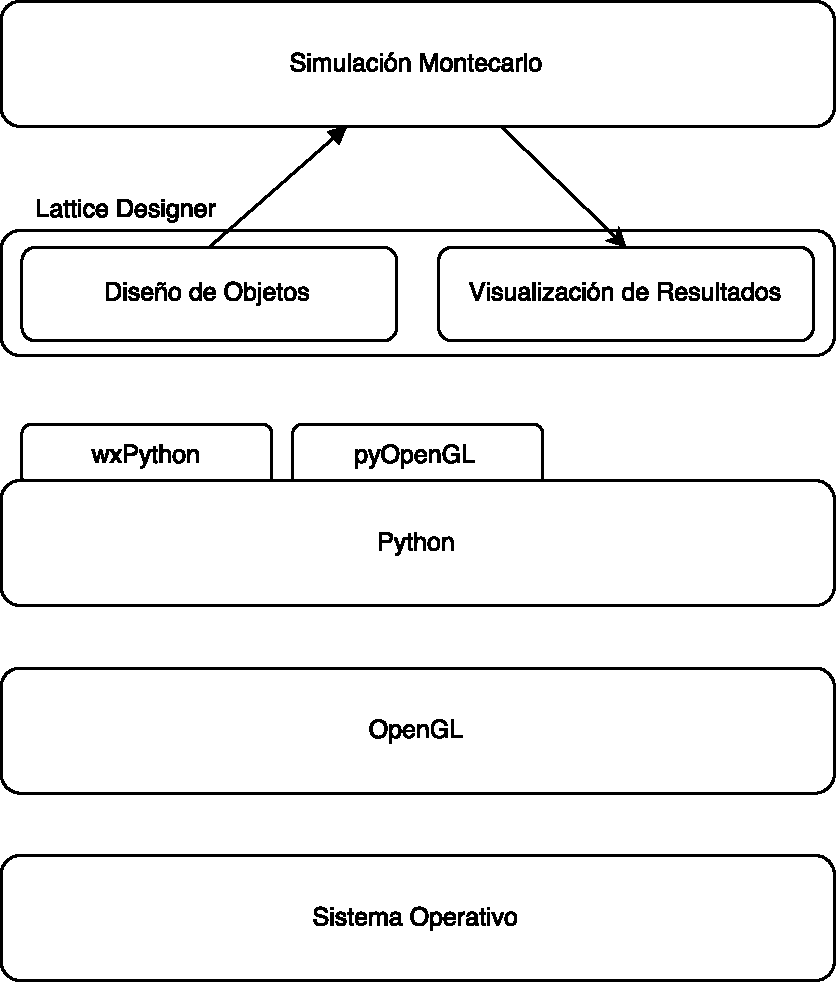
\includegraphics[scale=.7]{images/arquitectura}
  \caption{\em Diagrama de la arquitectura de la solución.}
  \label{arquitectura}
\end{figure}

\section{Sistema Operativo}

Si bien la aplicación fue desarrollada íntegramente en Mac OS X, y es por lo tanto el sistema operativo oficial de la presente memoria, todo el sistema fue desarrollado pensando en ser eventualmente multi-plataforma, sin que esta portación a distintos Sistemas Operativos tenga mayores complicaciones, más allá de los problemas que uno pueda encontrar por la distinta estructura de estos. Para esto tanto la elección del lenguaje de programación como de las distintas bibliotecas usadas fueron hechas teniendo el cuenta que deben poder ser ejecutados en los 3 sistemas operativos más usados, OS X, Windows y Linux.

\section{OpenGL}

Como parte importante del software es su capacidad de representar gráficamente en 3D tanto los átomos de un objeto diseñado como los resultados de las simulaciones, es necesario buscar una biblioteca de procesamiento gráfico 3D que fuera realmente multi-plataforma, tanto a nivel de sistema operativo como de tarjetas gráficas. Debido a esto se elige el estándar OpenGL, el cuál tiene implementaciones tanto para Windows, OS X y Linux, además de ser el estándar de la industria para gráficos 2D y 3D \citep{website:AboutOpenGL}. Esto permite tener una gran comunidad activa lo que a su vez se traduce en una gran cantidad de documentación al respecto.

La especificación del estándar OpenGL era dirigido por el consorcio independiente \emph{OpenGL Architecture Review Board} hasta el año 2006, cuando se decidió transferir esta responsabilidad al \emph{Khronos Group} \citep{website:OpenGLARB}, un consorcio formado por distintas organizaciones, tanto empresariales como académicas, quienes manejan múltiples estándares de la industria como \emph{OpenGL ES}, \emph{OpenCL} y \emph{WebGL} \citep{website:KhronosGroup}.

\section{Python}

Para el lenguaje de programación se barajó inicialmente la opción de C++ por las ventajas que conlleva trabajar a bajo nivel. No obstante debido a su inclinada curva de aprendizaje y complejidad he decidido usar Python, ya que es un lenguage que también cumple con las características necesarias para este desarrollo, como el ser multi-plataforma, y tener a disposición bibliotecas de manejo gráfico como su compatibilidad con la API OpenGL, de tal forma de centrar la complejidad del proyecto en las representaciones 3D.

Python es un lenguaje de programación de alto nivel, interpretado y orientado a objetos, desarrollado durante el año 1990 por Guido van Rossum, aunque actualmente es de código abierto y mantenido por su comunidad, la que es liderada por la \emph{Python Software Foundation}, quienes además resguardan los derechos de este.

Algunas de las características más conocidas de Python es su fácil sintaxis y su gran biblioteca estándar, la que cubre áreas como Protocolos de comunicación, Ingeniería de software e Interfaces de Sistema Operativo \citep{pythonFeatures}.

Durante el desarrollo se la aplicación se usaron distintas bibliotecas, siendo las dos más importantes wxPython y pyOpenGL.

\subsection{wxPython}

wxPython es una biblioteca de python que permite usar de forma nativa wxWidgets, un set de herramientas de código abierto, escrita en C++ y inicialmente escrito por Julian Smart y actualmente mantenida por la comunidad que permiten crear interfaces gráficas en distintas plataformas como Windows, OS X, iOS, Linux, entre otros. En este trabajo wxPython maneja todas las interacciones de los usuarios, además de casi todas las interfaces gráficas con excepción de los \emph{canvas} de OpenGL.

\subsection{pyOpenGL}

pyOpenGL es una biblioteca que permite la programación en OpenGL directamente desde python. Es multiplataforma y totalmente compatible con la biblioteca de interfaz gráfica usada (wxPython). Uno de los sub-paquetes de pyOpenGL usado en esta memoria es GLUT, la que permite crear fácilmente ciertos objetos en OpenGL, como esferas o conos, de tal forma de no tener que programar estos a partir de triángulos, como sería si se usara OpenGL puro.

\section{Lattice Designer}

Lattice Designer es el software desarrollado en esta memoria, el cual permite a científicos generar configuraciones atómicas sobre los cuales se simula la aplicación de campos electromagnéticos y la visualización de resultados generados por la simulación. Aunque esta herramienta está pensada para ser usada por investigadores del Departamento de Física de la Universidad de Santiago de Chile, la aplicación que ejecuta la simulación es usada por diversas organizaciones académicas, por lo que este software pretende ser un aporte a la comunidad científica en general.

Durante el desarrollo se puso especial énfasis en la experiencia de usuario, de tal forma que cualquier científico que tenga acceso a esta aplicación sea capaz de usarlo sin la necesidad de un entrenamiento; por este motivo el software tiene todos sus textos en inglés.

Como lo muestra la figura \ref{arquitectura}, la aplicación se compone de dos módulos claramente definidos: el diseño de configuraciones atómicas y la visualización de resultados de la simulación Monte Carlo.

\subsection{Diseño de configuraciones atómicas}

Para el desarrollo de esta funcionalidad se usó como base el sistema de diseño de objetos actual, basado en un mapa de bits, explicado en la sección \ref{intro:procesoactualmapa} de esta memoria, pero con la finalidad de que el proceso completo sea ejecutado en la misma aplicación disminuyendo con esto la probabilidad de errores que se puedan producir.

Dentro de las entradas de esta funcionalidad están tanto el mapa de bits, mediante una grilla binaria, como los distintos parámetros físicos asociados al objeto, como el tipo de estructura cristalina, la constante de red y el número de capas, entre otros (ver figura \ref{softwareDiseno}). Además se le ofrece al usuario mucha información dinámica, es decir, que va cambiando en base a los parámetros de entrada, como por ejemplo la constante de escalamiento.

\begin{figure}[ht]
  \centering
  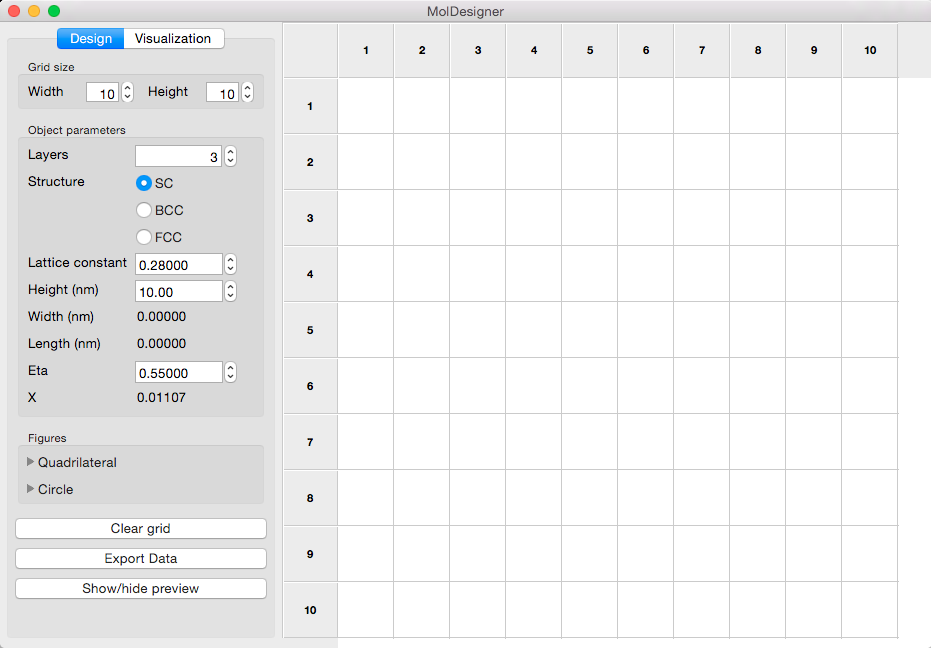
\includegraphics[scale=.45]{images/softwareDiseno}
  \caption{\em Vista de diseño de configuraciones atómicas del software}
  \label{softwareDiseno}
\end{figure}

Una de las características del diseño es la posibilidad de crear imágenes pre-definidas en base a dimensiones entregadas por el usuario. De esta forma se pueden crear cuadriláteros definiendo su ancho y alto o circunferencias con un radio específico. Una vez ingresados los parámetros solo es necesario hacer click en la posición de la grilla donde se quiere dibujar.

Como muestra la figura \ref{softwareDisenoPrevisualizacion}, el software permite también al usuario ver de forma inmediata la visualización 3D de la configuración atómica que se está creando con colores identificando sus distintos tipos de partículas, permitiendo así comprobar de manera rápida y fácil si efectivamente el diseño es el deseado.

\begin{figure}[ht]
  \centering
  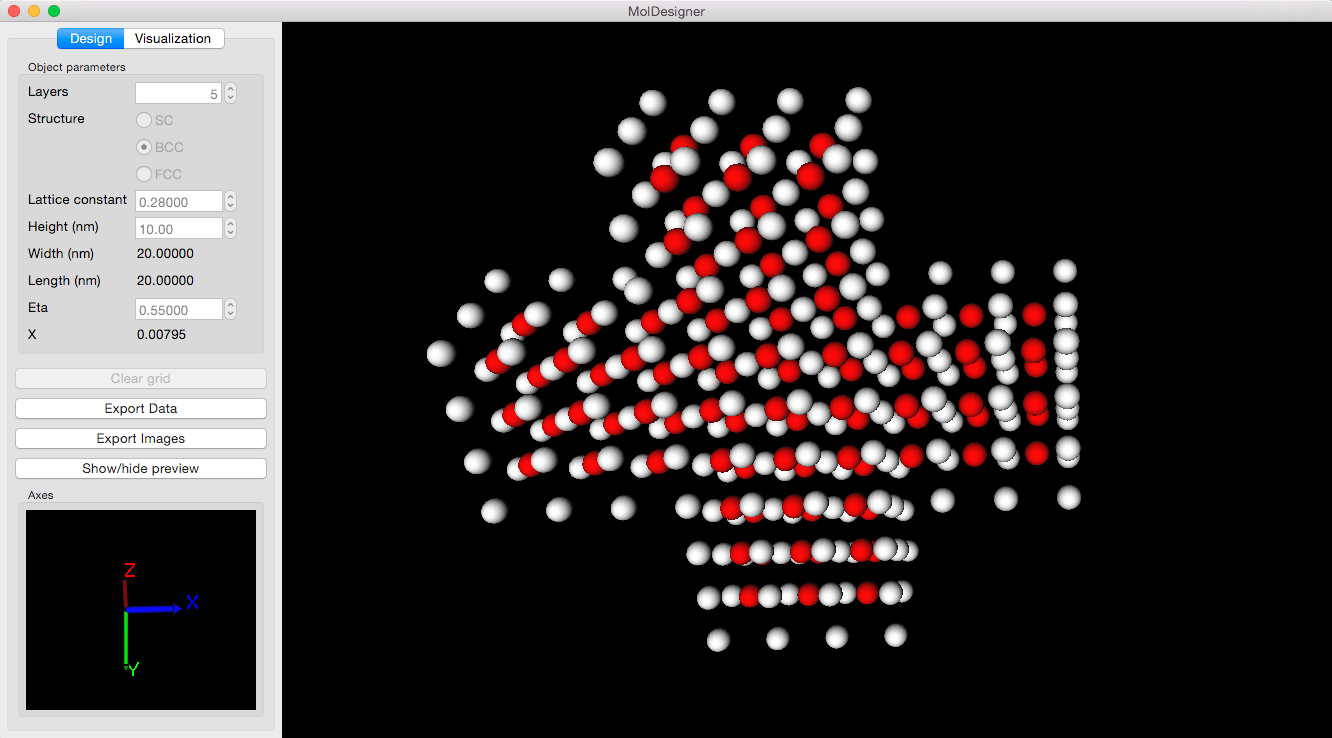
\includegraphics[scale=.35]{images/softwareDisenoPrevisualizacion}
  \caption{\em Previsualización de un objeto diseñado}
  \label{softwareDisenoPrevisualizacion}
\end{figure}

Una vez confirmado que el objeto diseñado es el deseado es posible exportar directamente las imágenes de la configuración atómica y los ejes coordenados para referencia; así como también el archivo que describe la configuración atómica, el que sirve como entrada para el software de simulación. A diferencia del proceso actual, donde el archivo exportado debe ser modificado para poder ser usado, en este caso los datos exportados puedes ser usados inmediatamente para ejecutar una simulación.

\subsection{Visualización de resultados}

El segundo módulo se basa específicamente en los requerimientos de los \emph{stakeholders}, sin tener un proceso actual como base, ya que esta es la gran debilidad que tienen actualmente.

Dentro de las funcionalidades de este módulo se encuentra la visualización y exportación del estado de la simulación en un tiempo \emph{t}, incluyendo los vectores de campo magnético, la curva de histéresis del campo magnético y los ejes coordenados para referencia. Estos son elementos que los científicos necesitan en sus publicaciones.

Las figuras \ref{softwareVisualizacionVectors}, \ref{softwareVisualizacionAxes} y \ref{softwareVisualizacionPlot} son las tres imágenes que se pueden exportar del estado de la simulación representado en la figura \ref{softwareVisualizacionPantalla}.


\begin{figure}[ht]
  \centering
  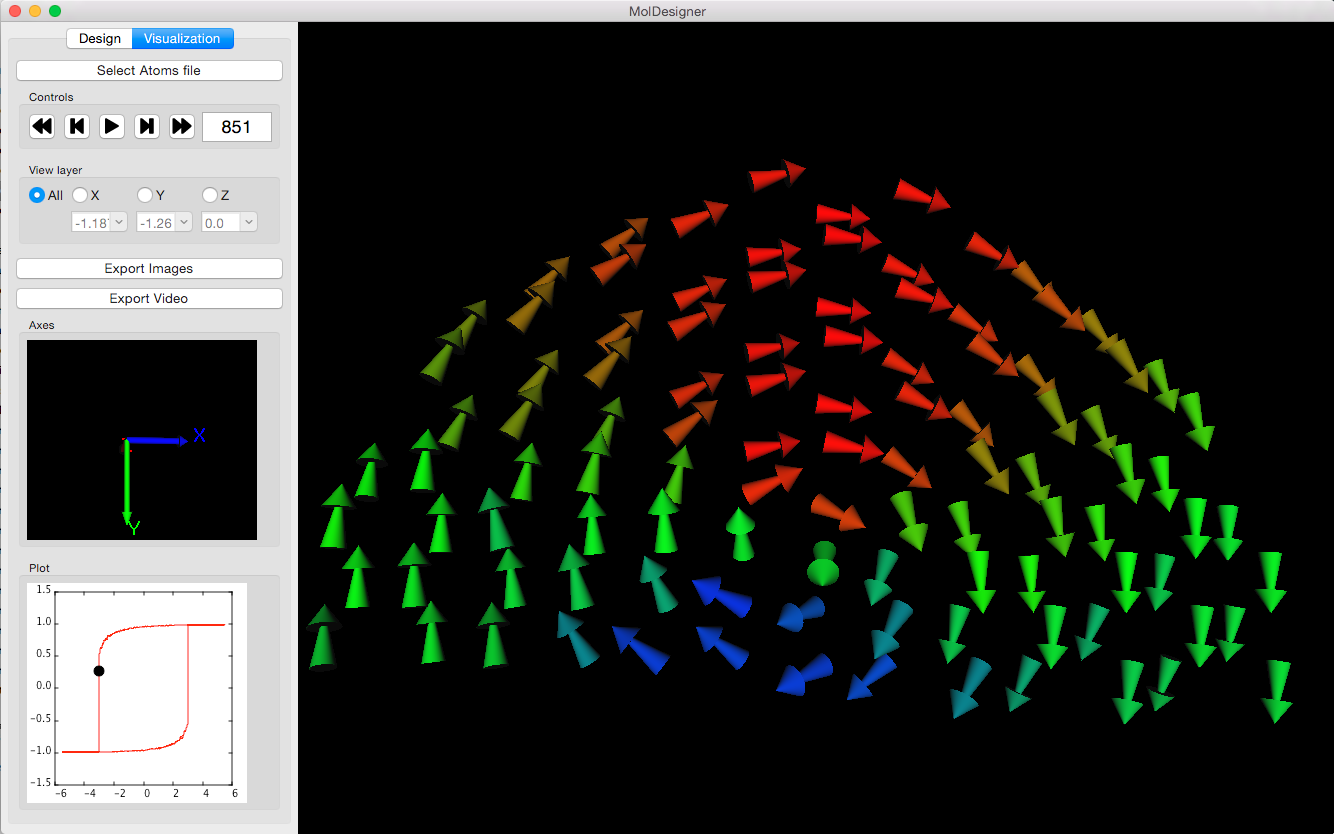
\includegraphics[scale=.3]{images/softwareVisualizacionPantalla}
  \caption{\em Pestaña de visualización de resultados en $t = 851$}
  \label{softwareVisualizacionPantalla}
\end{figure}


\begin{figure}[ht]
  \centering
  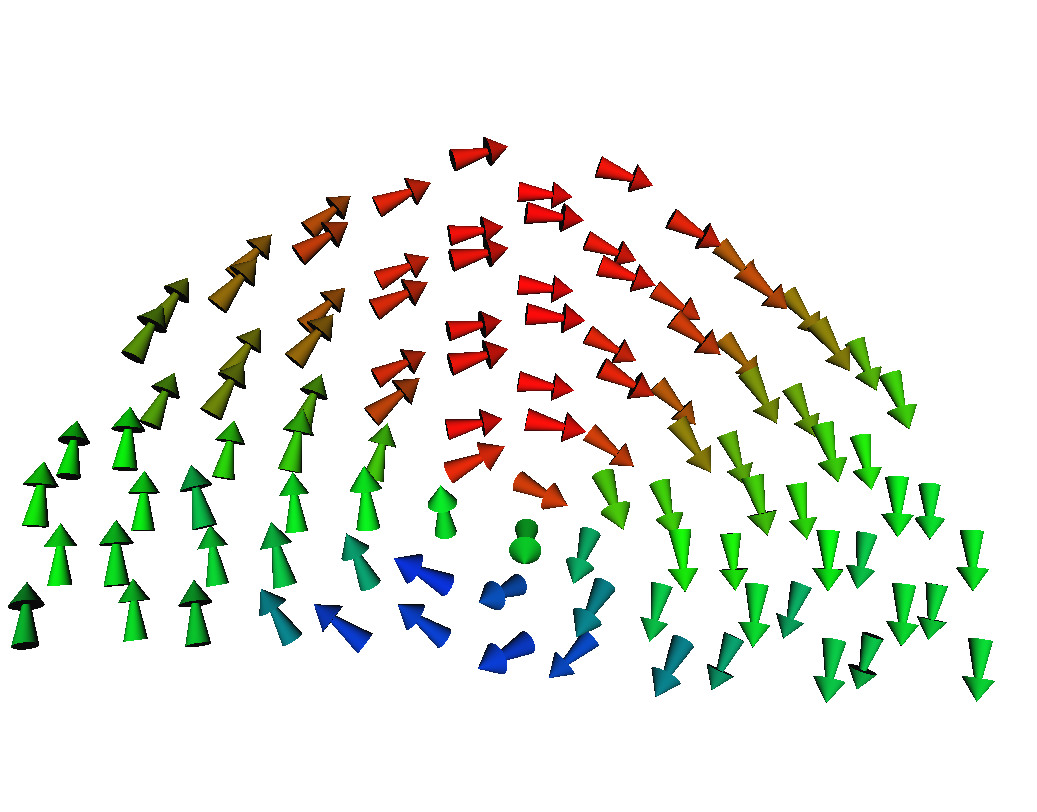
\includegraphics[scale=.3]{images/softwareVisualizacionVectors}
  \caption{\em Imagen de vectores exportada para publicación}
  \label{softwareVisualizacionVectors}
\end{figure}


\begin{figure}[ht]
  \centering
  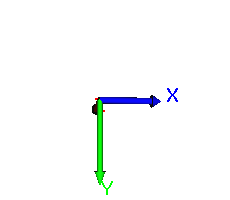
\includegraphics[scale=.6]{images/softwareVisualizacionAxes}
  \caption{\em Imagen de ejes de referencia exportada para publicación}
  \label{softwareVisualizacionAxes}
\end{figure}


\begin{figure}[ht]
  \centering
  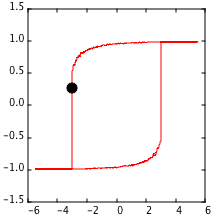
\includegraphics[scale=.6]{images/softwareVisualizacionPlot}
  \caption{\em Imagen de curva de histéresis exportada para publicación}
  \label{softwareVisualizacionPlot}
\end{figure}

Otras características disponibles es la asignación de colores para cada vector según uno de sus componentes cartesianos, usando una escala de colores de azul a rojo. En el caso de la figura \ref{softwareVisualizacionVectors} el máximo valor de $\hat{i}$ será rojo y el mínimo será azul. Esto permite identificar rápidamente una tercera dimensión en una imagen 2D y también los vortex que se generan.

También es posible ver la variación de los vectores a través del tiempo como video y luego exportarlo de tal forma que este pueda ser usado fácilmente en conferencias donde se divulguen los resultados.

Cabe notar que todas las características anteriores pueden ser ejecutadas mientras se visualiza solo una de las múltiples capas en la que se puede dividir el objeto, en base a cualquier eje coordenado, como se puede ver en las figuras \ref{softwareVisualizacionVectorsZ} y \ref{softwareVisualizacionVectorsX}.

\begin{figure}[ht]
  \centering
  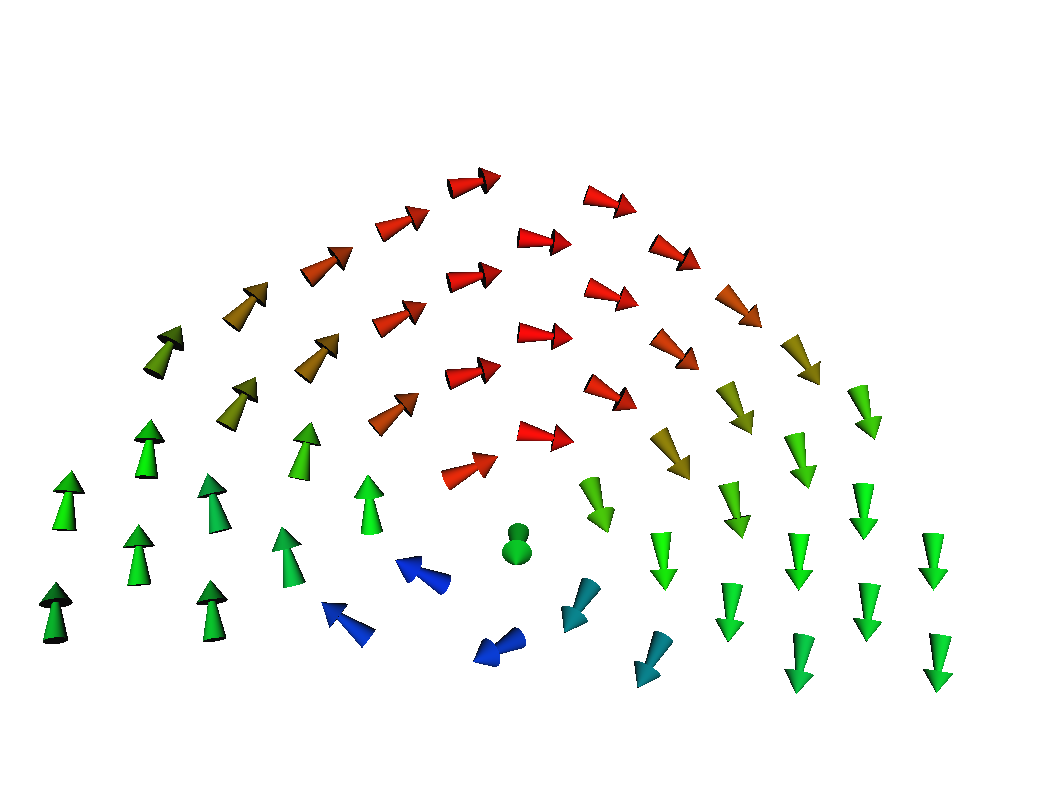
\includegraphics[scale=.3]{images/softwareVisualizacionVectorsZ}
  \caption{\em Estado de la simulación para t = 851 solo para la capa Z = 0}
  \label{softwareVisualizacionVectorsZ}
\end{figure}


\begin{figure}[ht]
  \centering
  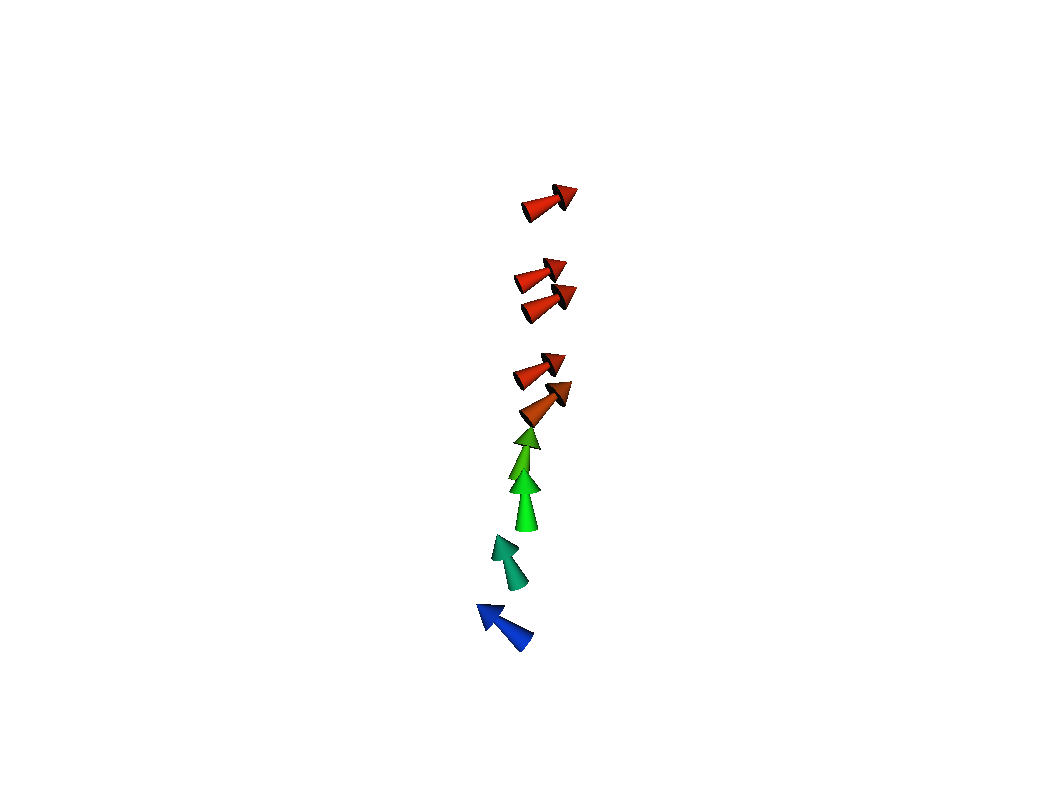
\includegraphics[scale=.3]{images/softwareVisualizacionVectorsX}
  \caption{\em Estado de la simulación para t = 851 solo para la capa X = -0.395}
  \label{softwareVisualizacionVectorsX}
\end{figure}